\label{ch:AnalyzingGraphs}

\begin{jointwork}
	In this chapter, we will put the tools and workflows described in the previous sections to the use. We will train two different Reinforcement-Learning Agents on different marketplaces, and then monitor them using all of the tools at our disposal, highlighting where each tool is most useful, and what could be improved.
\end{jointwork}

\section*{Setting up the experiments}

We will first be conducting two different experiments, using two different Reinforcement-Learning algorithms and two different market environments. Both experiments will however be conducted on the same marketplace type, a Circular Economy model with rebuy-prices. Both experiments will be conducted multiple times using the same configurations\todo{Why?}, and diagrams of different versions will be denoted using an underscore for differentiation.

\subsection*{SAC-Duopoly}

For the first experiment, we will train a Reinforcement-Learning Agent using the SAC-algorithm~\cite{StableBaselines3SAC} on a Duopoly marketplace with rebuy prices. The agent will be trained against a Rule-Based agent, more specifically the \emph{RuleBasedCERebuyAgentStorageMinimizer}, as presented in \nameref{subsec:DataDrivenModels}. The concrete configurations can be found in \Cref{fig:SACDuopolyConfigEnvironment} and \Cref{fig:SACDuopolyConfigMarket}. We will refer to this experiment as the \emph{SAC-Duopoly}.

\subsection*{PPO-Oligopoly}

For the second experiment, we will be training a different Reinforcement-Learning agent on a more complex market with more participants: A PPO-agent~\cite{StableBaselines3PPO} will be trained on an Oligopoly-Scenario, again with rebuy prices enabled. Three different Rule-Based agents will compete against the PPO-Agent on the same market:

\begin{enumerate}
	\item A \emph{FixedPriceAgent}, which will always set the following three prices:
	      \begin{itemize}
		      \item New price: 7
		      \item Refurbished price: 4
		      \item Rebuy price: 2
	      \end{itemize}
	      It should be noted that the configured maximum possible price is 10, which can also be configured using the configuration files. Depending on this maximum price, the prices set by \emph{FixedPriceAgents} must be adjusted to allow them to realistically compete in the market.
	\item The second agent is a \emph{RuleBasedCERebuyAgentCompetitive}, a more complicated and sophisticated version of the simple \emph{RuleBasedCEAgent}, which was introduced in \nameref{subsec:InventoryBasedModels}. The competitive version used for this experiment combines features of both the basic \emph{RuleBasedCEAgent} and the \emph{RuleBasedCERebuyAgentStorageMinimizer}. It's policy implementation can be found in \todo{Insert code snippet in Appendix}xyz.
	\item For the third competitor, we will again be using the \emph{RuleBasedCERebuyAgentStorageMinimizer}.
\end{enumerate}
This experiment will be referred to as the \emph{PPO-Oligopoly}.

\section*{Experiment results}

In the following sections we will use our different monitoring tools on the two experiments we conducted. We will start with the Live monitoring tools, which runs automatically after the training run and creates over 90 graphs and diagrams already. Due to this high number of available diagrams, we will always only look at a curated selection, highlighting those with the most and least use for the user.

\subsection*{Live monitoring}

\begin{figure}[!hbt]
	\begin{subfigure}{\textwidth}
		\centering
		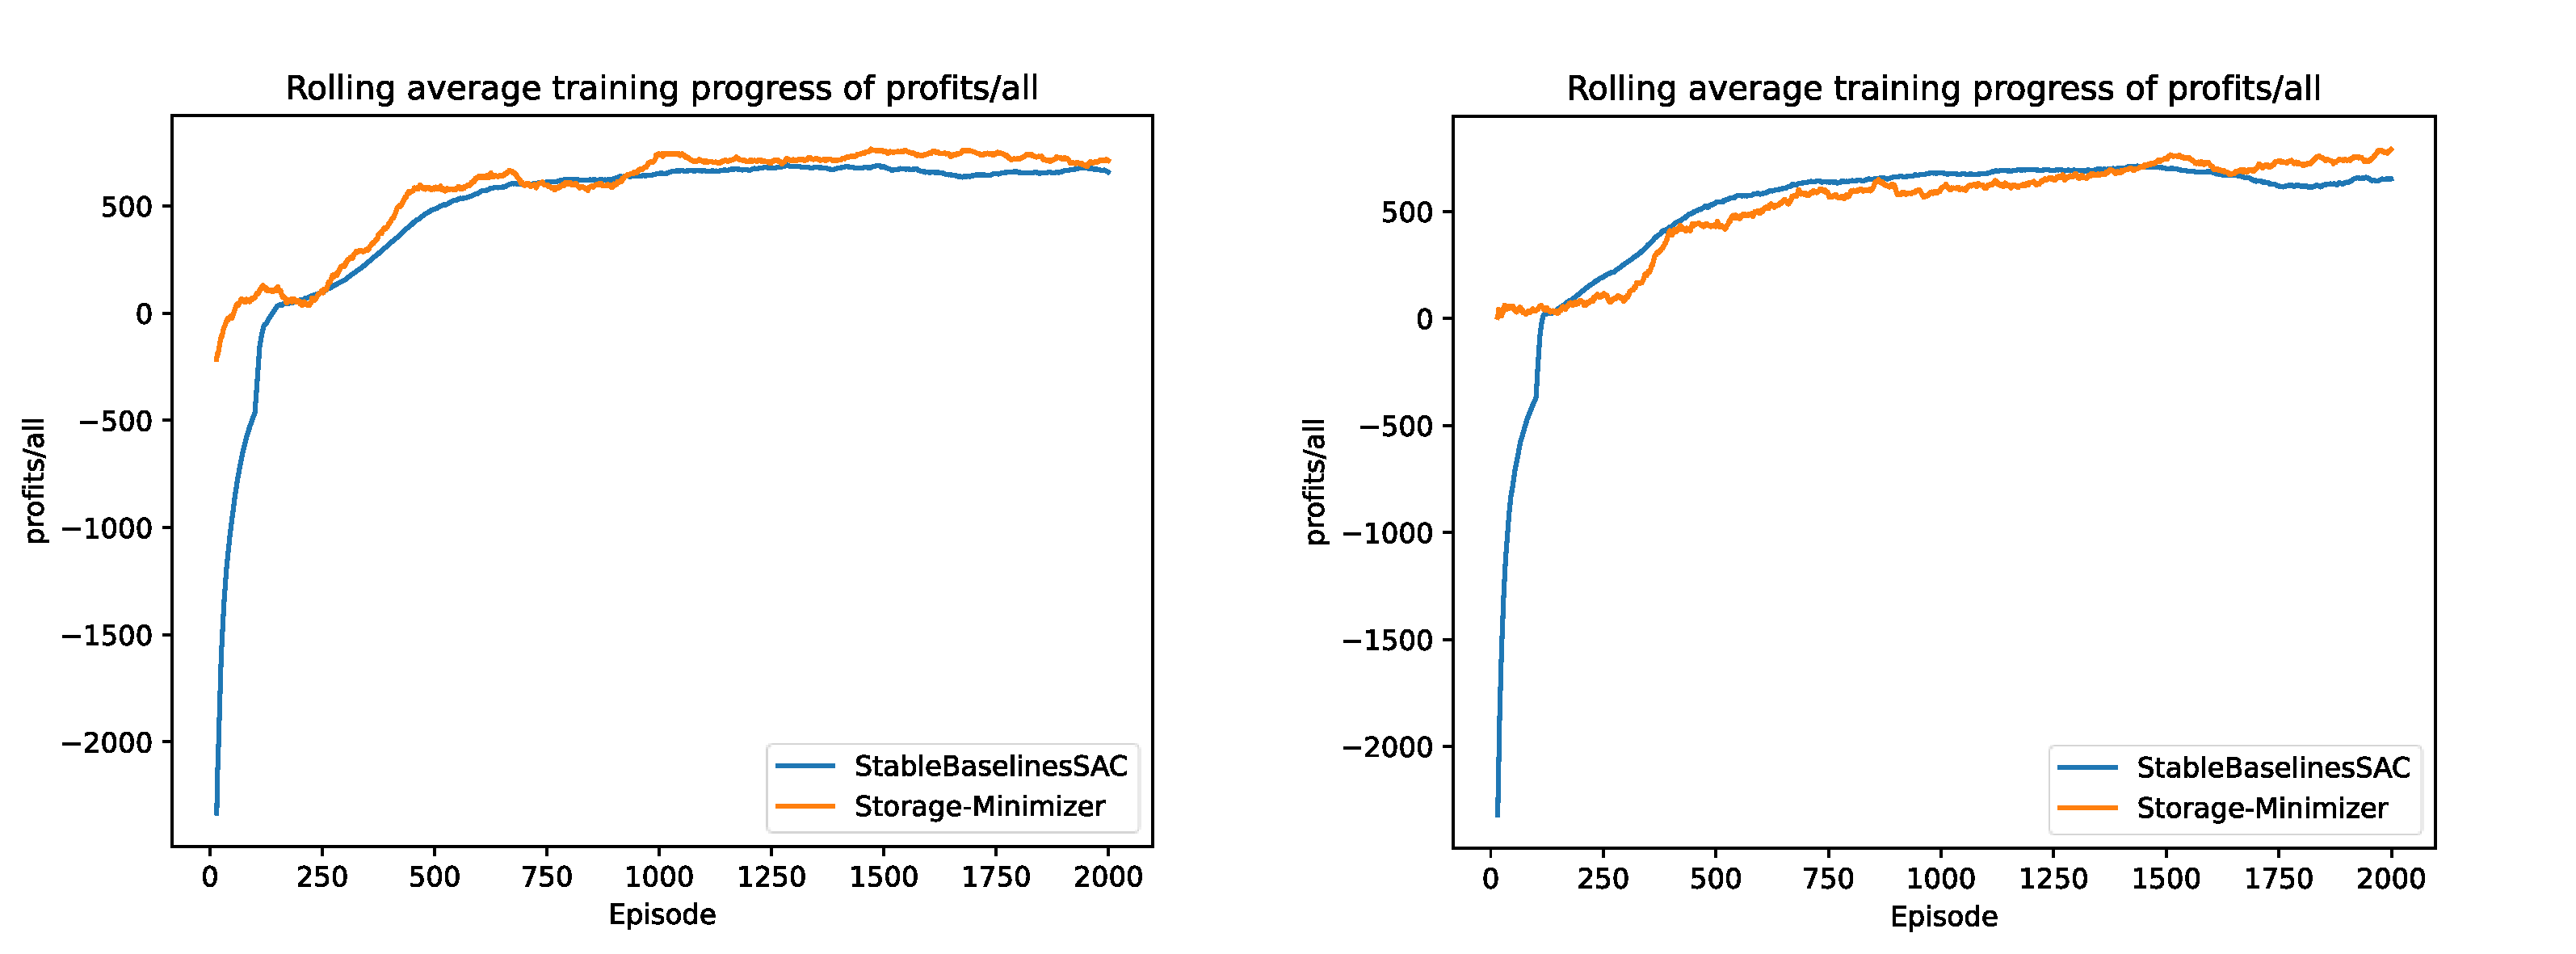
\includegraphics[width = \textwidth]{images/experiments/SACDuopoly/SACDuopolyProfits1_2.pdf}\\[1 ex]
	\end{subfigure}
	\begin{subfigure}{\textwidth}
		\centering
		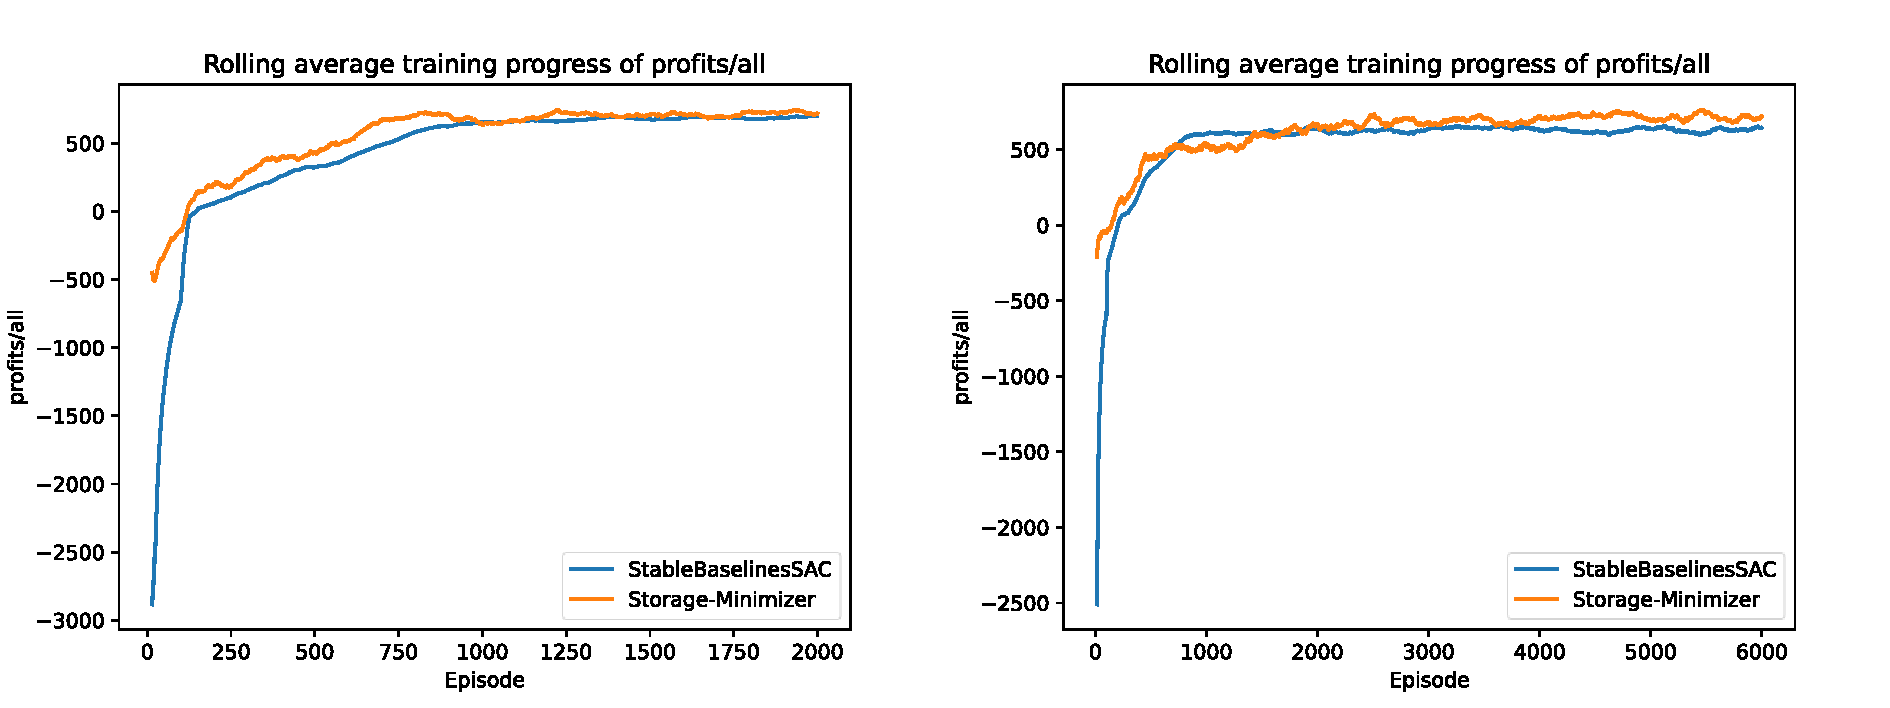
\includegraphics[width = \textwidth]{images/experiments/SACDuopoly/SACDuopolyProfits3_4.pdf}\\[1 ex]
	\end{subfigure}
	\caption{Profit per episode of four different training runs of an SAC-Agent on a Duopoly market. The agent in bottom right was trained using three times as many episodes as the other ones.}\label{fig:SACDuopolyProfitsMean}
\end{figure}

\todo{Split the diagrams into four different ones to allow for more distinct references later on}A commonly asked question when deciding on the quality of a Reinforcement-Learning Agent is their \emph{stability}\todo{cite?}. If an algorithm is stable, the trained agent will produce similar results over multiple training sessions, on the condition that the parameters do not differ. Not only the rewards achieved at the end of the training will be very similar, but also the amount of episodes needed to reach certain thresholds. In the case of the SAC-Duopoly experiment, we ran the same configuration four times: The first three experiments were run using the exact same parameters, for the fourth experiment the amount of training episodes were tripled, meaning that the SAC-Agent had more time to alter its policy. \Cref{fig:SACDuopolyProfitsMean} shows the results of these four training sessions, created using the \nameref{subsec:LiveMonitoring} tool and visualizes the data collected during the training process. Although many other graphs are created\todo{Table/List of all graphs needed}, the visualization of the total profit of the agent is the most convenient to use when evaluating an agent's performance, as the total profit is the parameter which the agent is trying to optimize.

\Cref{fig:SACDuopolyProfitsMean} shows the stability of the SAC-Agent very well. The agent not only reached the break-even threshold of a reward of 0 after around 150 episodes in each of the four training runs, but no matter the total length of training, the profit would always stabilize and stay at around 670. Had the monitoring tools shown that the agent performs worse than expected in some of the experiments, we could conclude that this particular algorithm is not fit for the type of work required by our market simulation.

We can also observe that the profits of the SAC-Agent and the Rule-Based Agent (in the case of this experiment, a \emph{RuleBasedCERebuyAgentStorageMinimizer}) seem to be closely linked to each other in this particular scenario. In the beginning of each experiment, when the Reinforcement-Learning agent still knows very little about the market and makes great losses, the Rule-Based agent also has a hard time to perform well. However, as soon as the SAC-Agent starts to perform better, the Rule-Based agent is also able to increase its mean profits at around the same rate as the SAC-Agent. Even more interestingly, the agents not only increase their profits at the same rate, but also very quickly arrive at a point where they earn the same mean amount as the other.

This might lead one to believe that the two competitors' policies align closely with each other. To validate this claim, another type of diagram created by the Live monitoring tool can be used: The density plots. These diagrams visualize probability densities for the various datasets recorded. While the diagrams shown in \Cref{fig:SACDuopolyProfitsMean} simply visualize data that was collected during the training run, density plots are created by simulating the marketplace an additional time.\todo{This is explanatory, perhaps move it to the approaches chapter} This allows us to use the `intermediate' models we saved during the training run (see \nameref{subsec:LiveMonitoring}) to compare the Reinforcement-Learning Agent's policies at different points in time during the training.

\begin{figure}
	\begin{subfigure}{\textwidth}
		\centering
		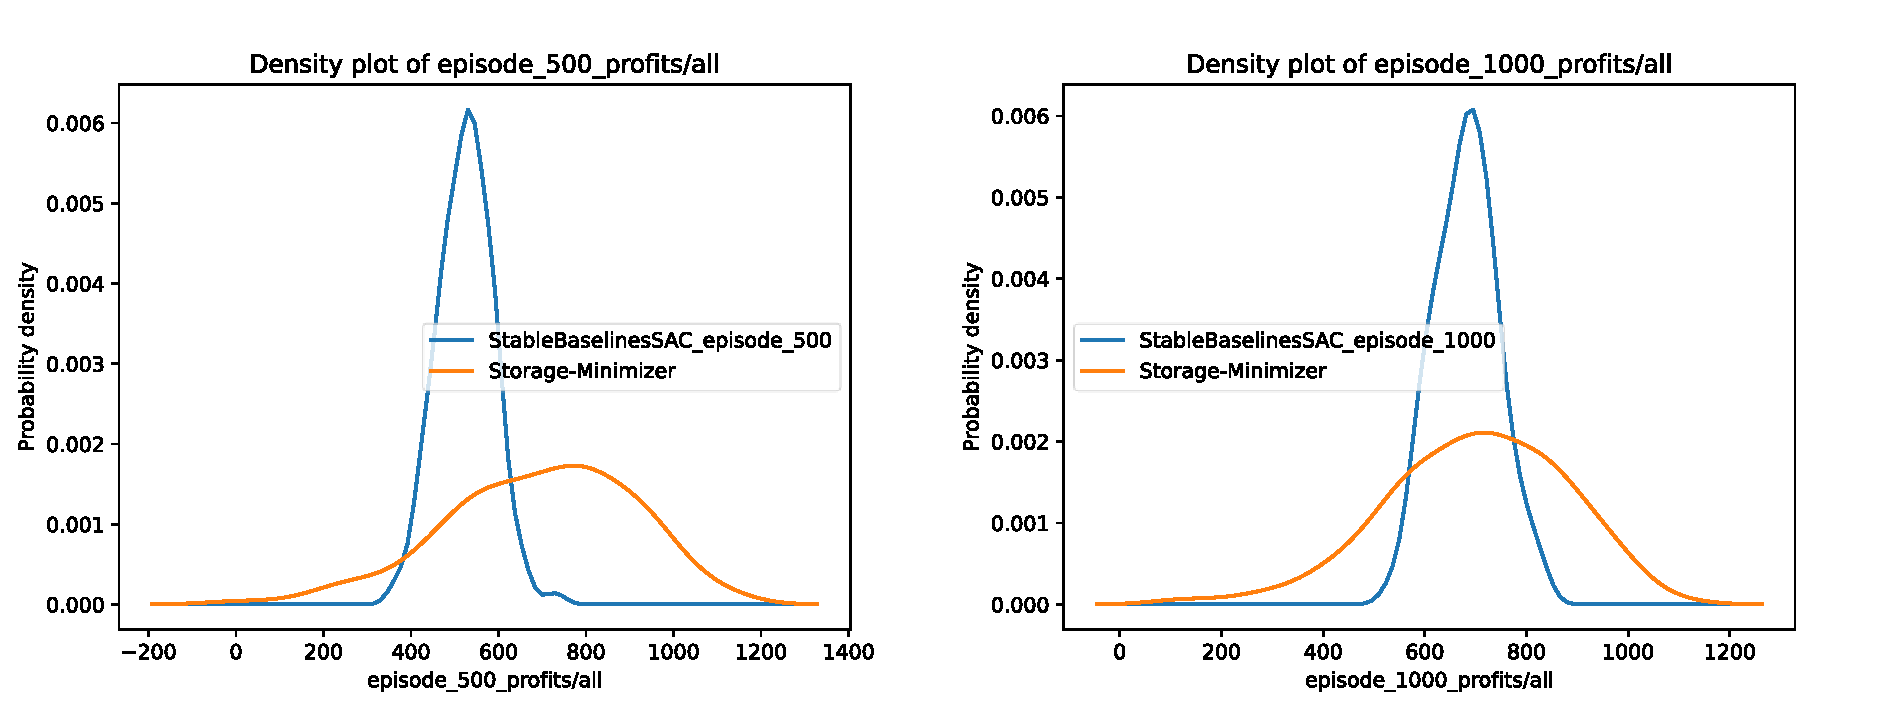
\includegraphics[width = \textwidth]{images/experiments/SACDuopoly/SACDuopolyProfitsDensity1_2.pdf}\\[1 ex]
	\end{subfigure}
	\begin{subfigure}{\textwidth}
		\centering
		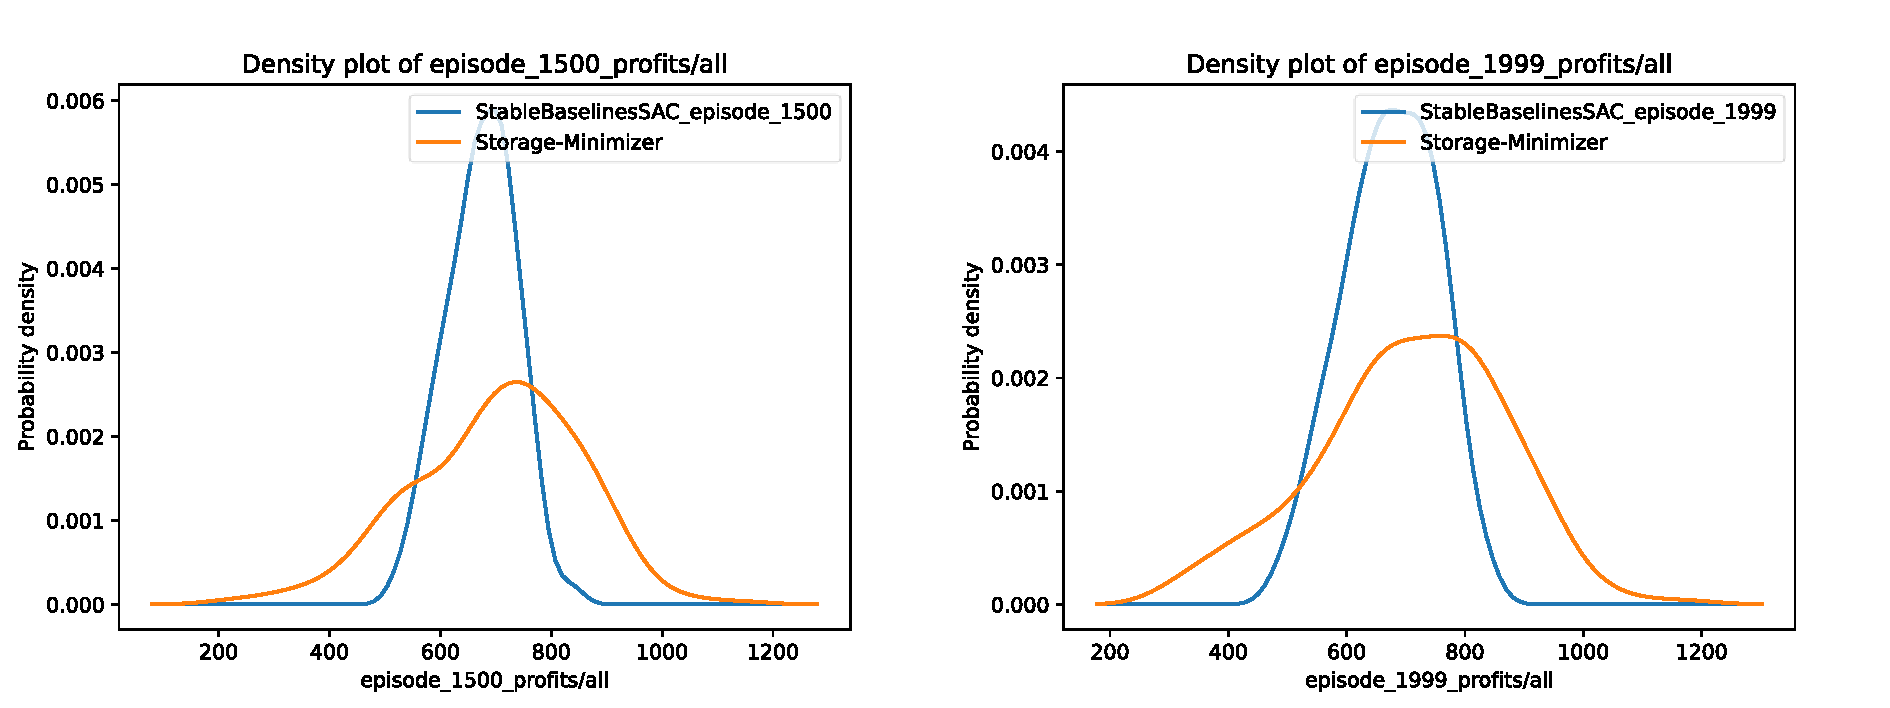
\includegraphics[width = \textwidth]{images/experiments/SACDuopoly/SACDuopolyProfitsDensity3_4.pdf}\\[1 ex]
	\end{subfigure}
	\caption{Probability densities for achieving a certain profit for four different training stages of the SAC-Duopoly\_1 experiment. The postfix of the agent name denotes the episode after which the model was saved.}\label{fig:SACDuopolyProfitsDensity}
\end{figure}

\Cref{fig:SACDuopolyProfitsDensity} shows the density plots of profit-per-episode for four different training stages of the SAC-Duopoly\_1 experiment. It can be concluded that the claim that the two agents' policies align closely is incorrect. Even though the mean reward within an episode is in many cases similar, the SAC-Agent achieves rewards which lie closer together, while the Rule-Based agent's rewards have more of a spread.

We can also observe that the SAC-Agent models which were trained for longer are not necessarily better or even the same quality of the earlier models. There is a significant improvement going from the model trained on 500 episodes to the one trained on 1000 episodes, this shift in the probability density curve can be correlated with the maximum mean rewards the two models could achieve during the training: For the model trained on 500 episodes, this was around 480, for the other it was about 650 (see \Cref{fig:SACDuopolyProfitsMean}). Both of these values have the respective highest probability of being achieved during the second simulation, as visualized as high points in the density plots. Going from the model trained on 1000 episodes to the next one, trained on 1500 episodes, both the probability densities as well as the mean rewards stay very close to each other. From this we can conclude that training the SAC-Agent for more than 1000 episodes is very likely to not have an effect on the maximum performance achievable by the algorithm. Going from the model trained on 1500 episodes to the last one, saved at the end of the training, we can however see a deterioration in performance: While the mean rewards hardly changed (\Cref{fig:SACDuopolyProfitsMean}), the probability density curve got wider at its base, extending out further towards a reward of 400, and lowering the high point at a reward of about 700 from the previous 0.6\% to only 0.4\%. This means that the model which was trained for the longest time produces less predictable results than those trained less, which may at first seem counterintutitive, but is a common phenomenom known as \emph{Catastrophic Forgetting} (see also \cite{CatastrophicForgetting}). The insights gained by our monitoring tools combined with the fact that we save `intermediate' models of the Reinforcement-Learning agent during training allows us to find the optimal trained model to use for further investigation and eventual deployment on the real market.

\section*{Which graphs are how useful?}
\section*{What limitations are there?}
\section*{What can we do in the future to improve the graphs or the workflow?}
\section*{Can we see which hyperparameters influence the results in what ways using the diagrams?}
\section*{How can we improve the workflow (e.g. Grid-Search) with our analysis?}

